\subsection{Geheugenbeheer in Linux}

Deelt veel kenmerken met UNIX, maar is beetje complexer. 

Hierbij heb je twee hoofdkenmerken:

\begin{itemize}
\item Proces virtueel geheugen
\item Toewijzing van kernelgeheugen.
\end{itemize}

\subsubsection{Virtueel geheugen in Linux}

Linux maakt gebruik van een paginatabelstructuur met drie niveaus, die bestaat uit de volgende soorten tabellen:

\begin{itemize}
\item Paginadirectory: Elke tabel is de grootte van een pagina, ieder actief proces heeft er een. Iedere ingang in deze directory wijst naar één pagina in de paginatussendirectory. Deze directory van een actief proces moet aanwezig zijn in het hoofdgeheugen.
\item Paginatussendirectory: Deze tussendirectory kan meerdere pagina’s omvatten. Iedere ingang wijst naar één pagina in de paginatabel.
\item Paginatabel: De paginatabel kan ook meerdere pagina’s omvatten. Iedere ingang wijst naar één virtuele pagina van het proces.
\end{itemize}

\begin{figure}[htp]
    \centering
            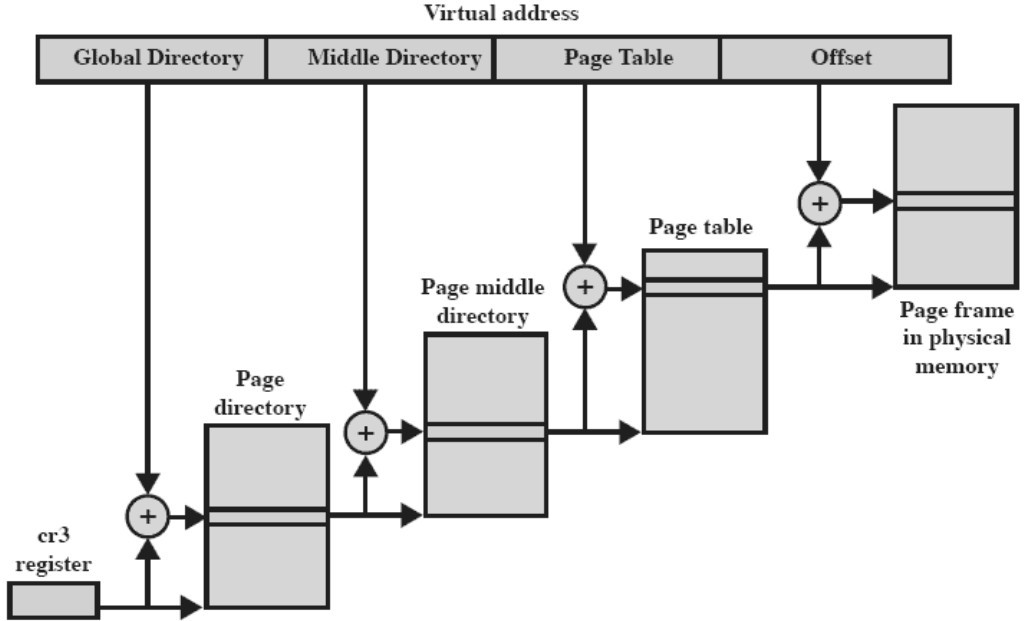
\includegraphics[width=4in]{img/adresvertalinglinux}
        \caption{Adresvertaling in Linux}
    \label{fig:Adresvertaling in Linux}
\end{figure}

Een adres in virtueel adres in Linux bestaat uit 4 velden:

\begin{enumerate}
\item De index van de paginadirectory
\item De index van de paginatussendirectory
\item De index van de paginatabel
\item De offset binnen de gekozen geheugenpagina
\end{enumerate}


\textbf{Paginavervanging}

Het is gebaseerd op het klok algoritme, maar de use bit is vervangen door een 8-bit age variabele. Deze wordt verhoogd met elke pagina acces. Het systeem zelf verlaagt de use bit periodiek. Wanneer een pagina een leeftijd heeft van 0 is het een kandidaat voor paginavervanging.

Dit is ook wel een vorm van Least Frequently Used strategie.
